\plain{Visão Geral}

\section{Visão Geral do Sistema}

\begin{frame}
    \frametitle{Visão Geral do Sistema}

    Quatro etapas principais:

    \begin{itemize}
        \item Obter \alert{informação sobre a fase}
        \item \alert{Detectar a fase} corretamente
        \item \alert{Variação de Frequências} (HMFCW)
        \item \alert{Cálculo da posição 3D}
    \end{itemize}
\end{frame}

\begin{frame}
    \frametitle{Visão Geral do Sistema}

    \begin{center}
        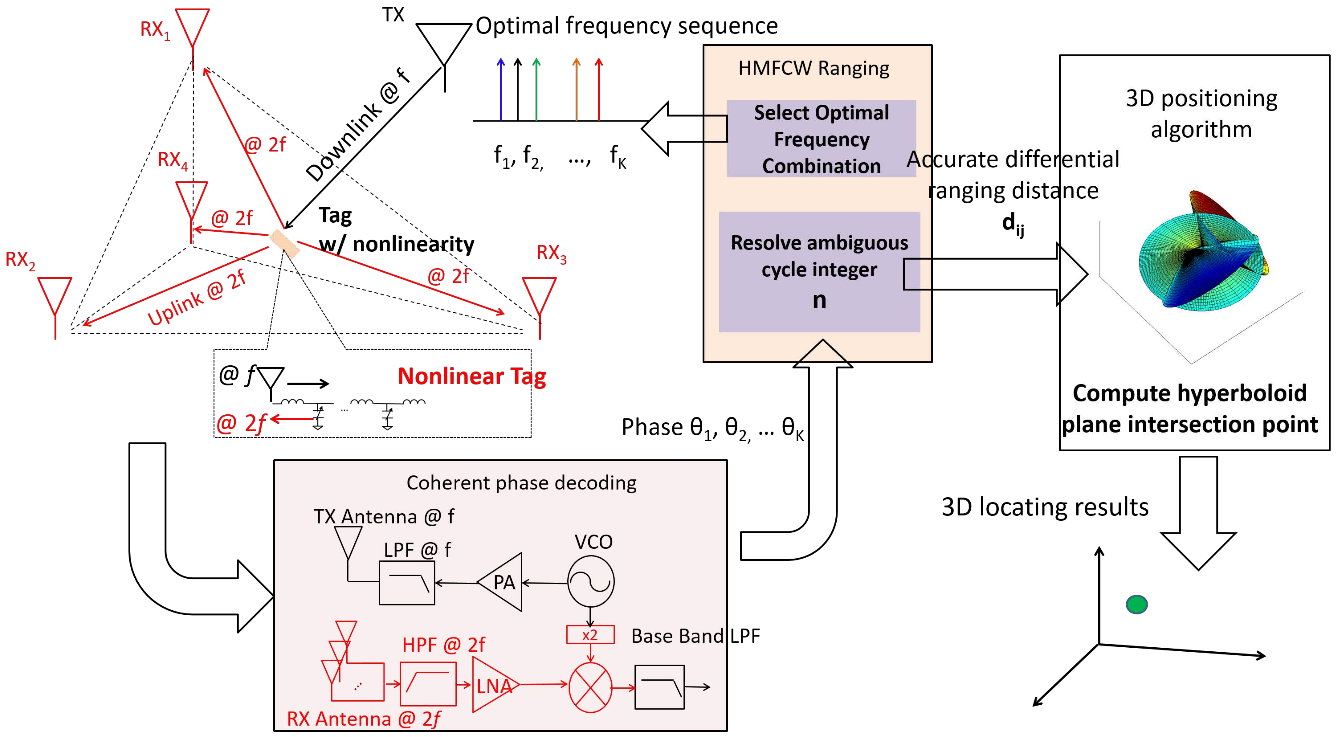
\includegraphics[width=1\textwidth]{overview}
    \end{center}
\end{frame}

\plain{Localização 3D}
\section{Soluções para Localização 3D}

\subsection{Eliminando o Auto-Bloqueio}

\begin{frame}
    \frametitle{Eliminando o Auto-Bloqueio}

    Entendendo o problema:
    \begin{itemize}
        \item Tags RFID consomem \alert{$\approx{}10\mu{}W$}
        \item Não têm energia para \alert{gerar sinais}
        \item Portanto, precisam \alert{refletir o sinal do emissor}
            \pause
        \item \alert{Como saber de onde vem uma reflexão?}
    \end{itemize}
\end{frame}

\begin{frame}
    \frametitle{Eliminando o Auto-Bloqueio}

    \begin{center}
        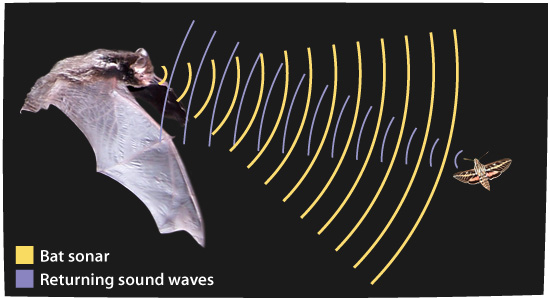
\includegraphics[width=.6\textwidth]{echolocation}
    \end{center}

    \pause
    \begin{columns}[T,onlytextwidth]
        \column{.25\textwidth}
        \begin{center}
            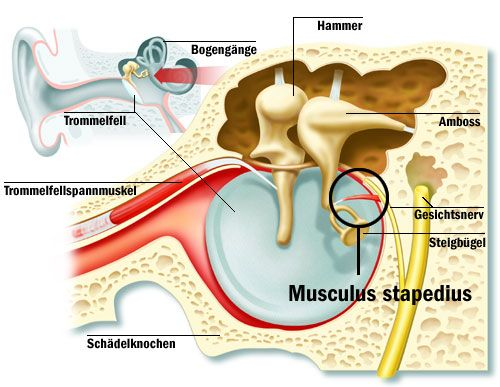
\includegraphics[width=\textwidth]{stapedius}
        \end{center}

        \pause

        \column{.25\textwidth}
        \begin{center}
            \vfill
            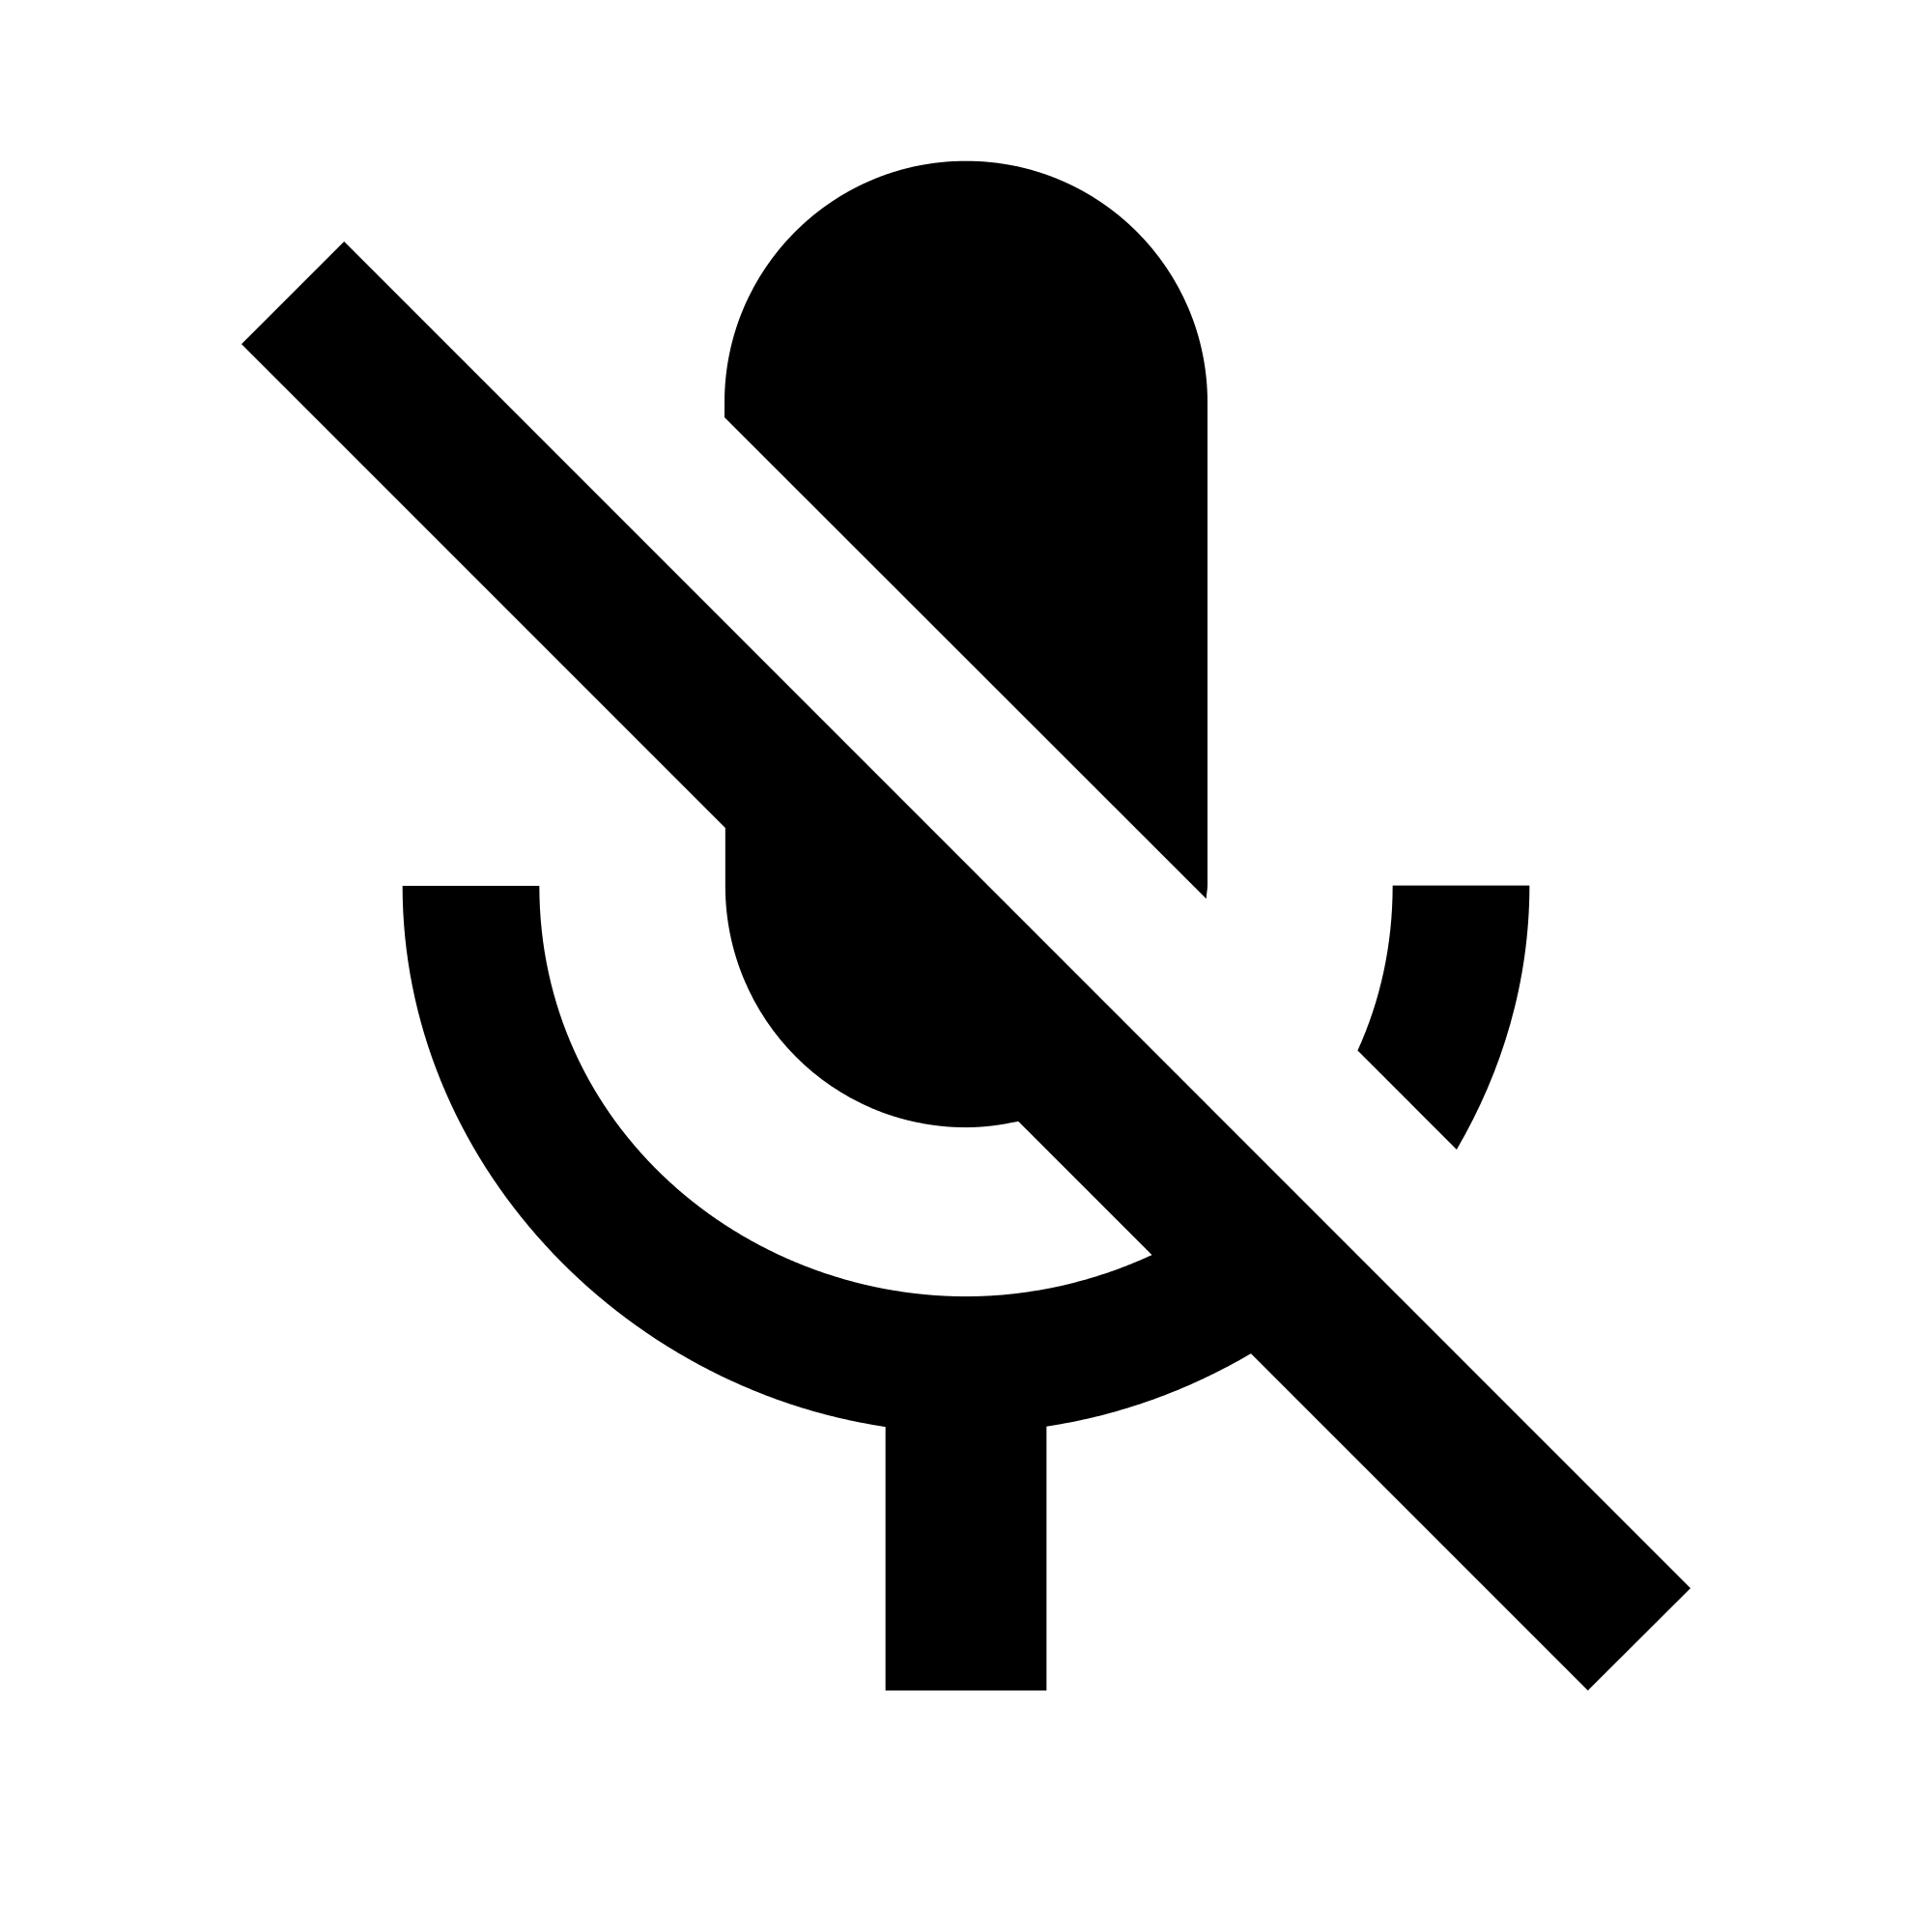
\includegraphics[width=.8\textwidth]{mute}
        \end{center}

        \pause

        \column{.25\textwidth}
        \begin{center}
            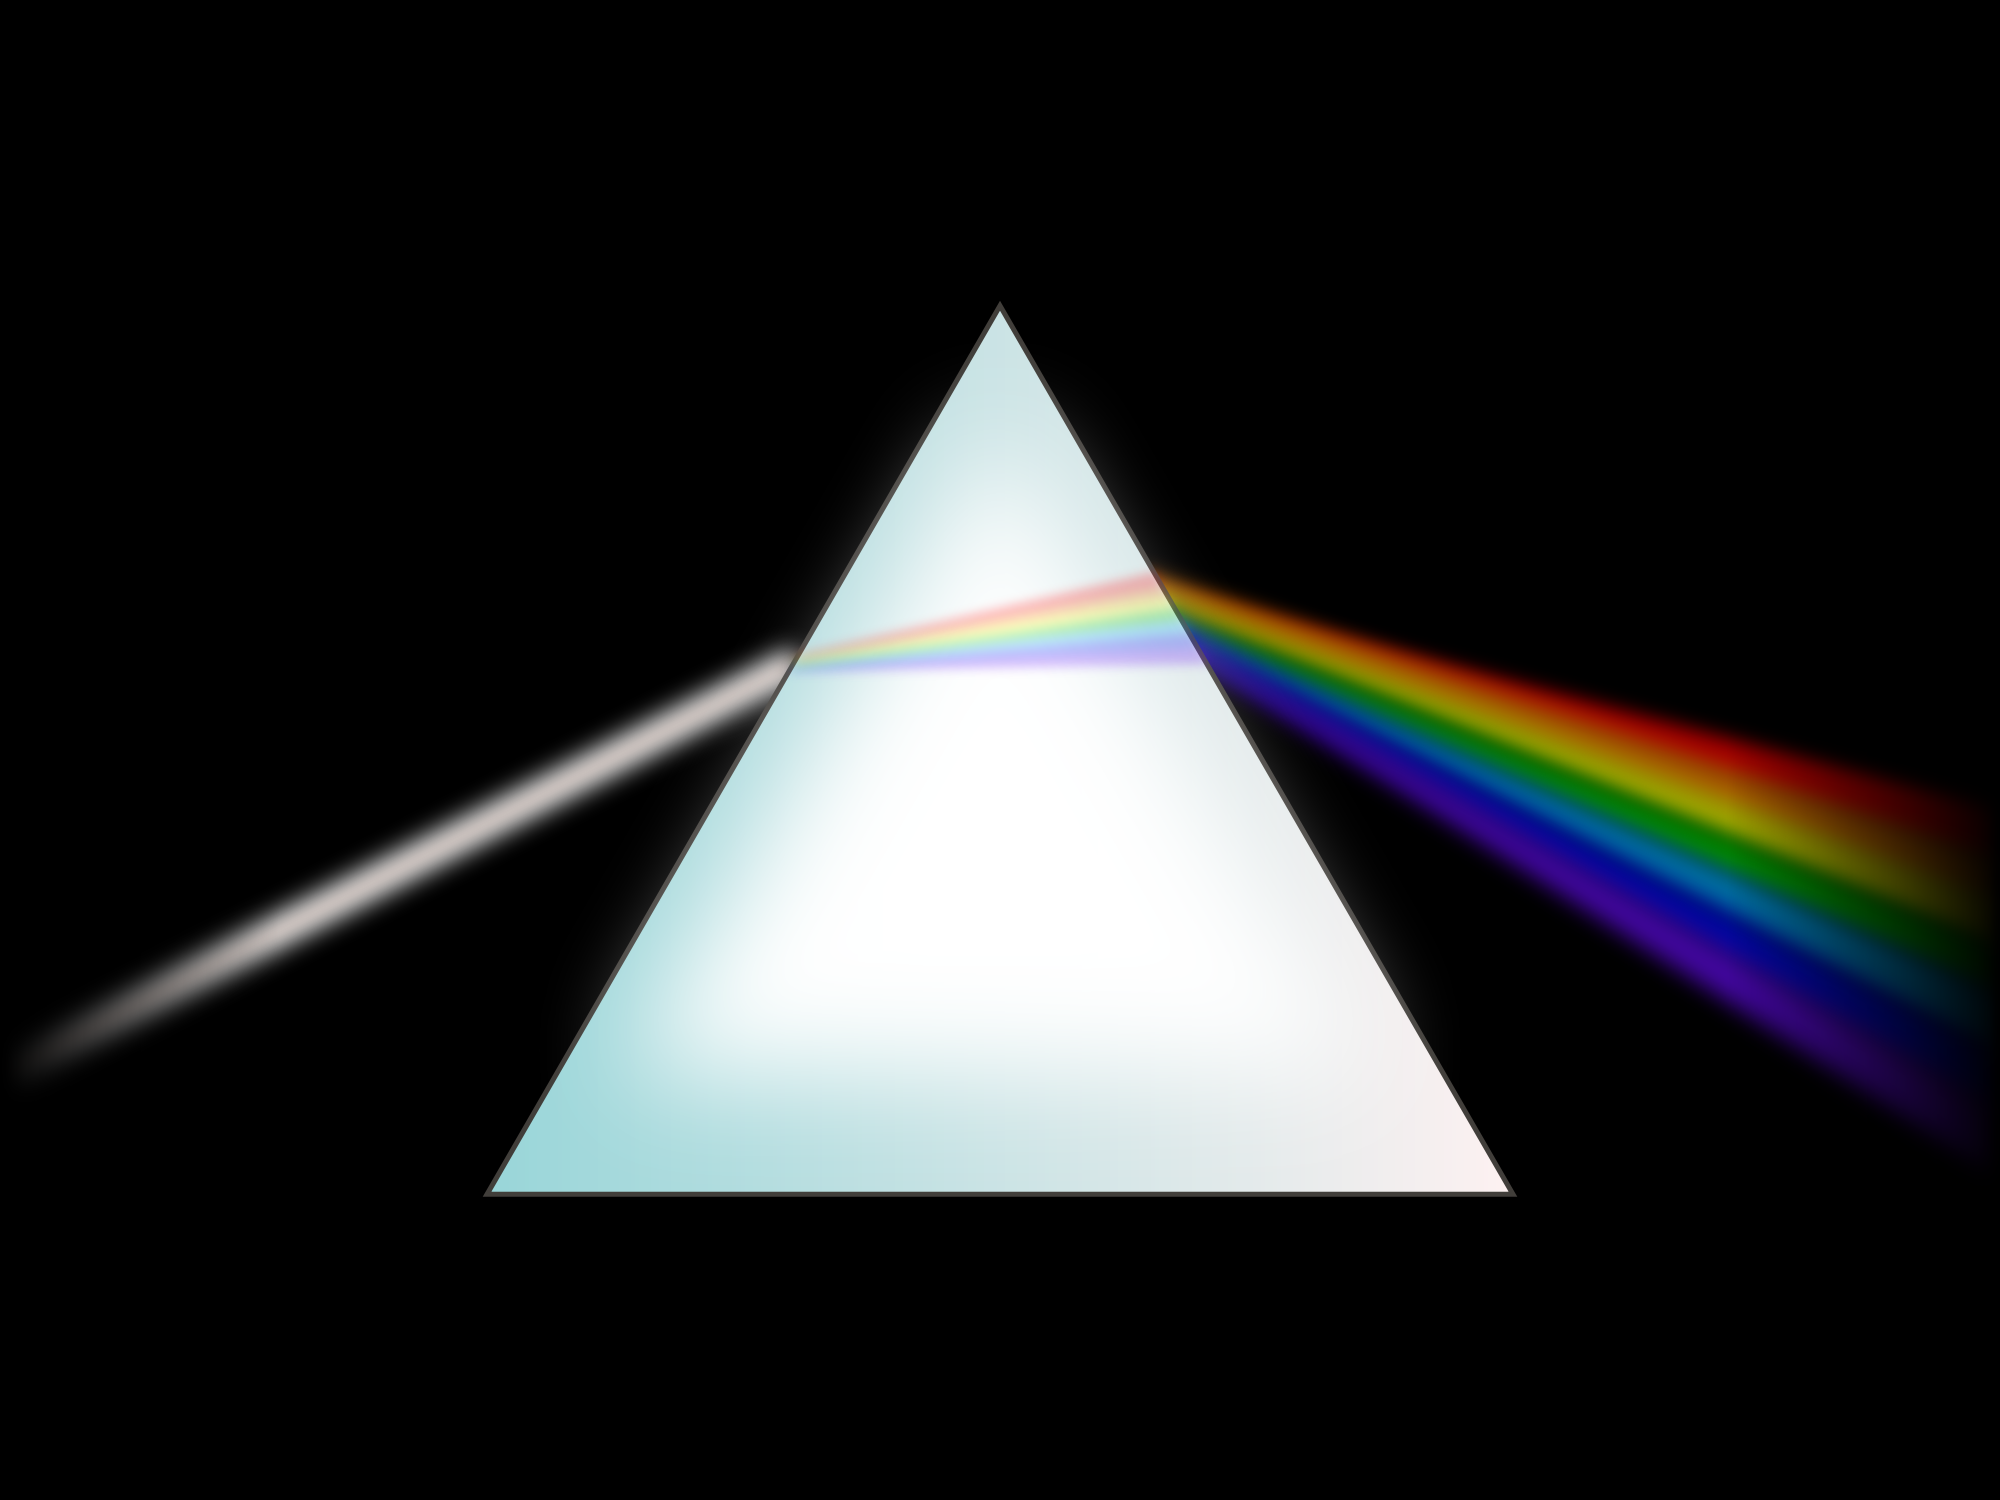
\includegraphics[width=1\textwidth]{spectrum}
        \end{center}

        \pause

        \column{.25\textwidth}
        \begin{center}
            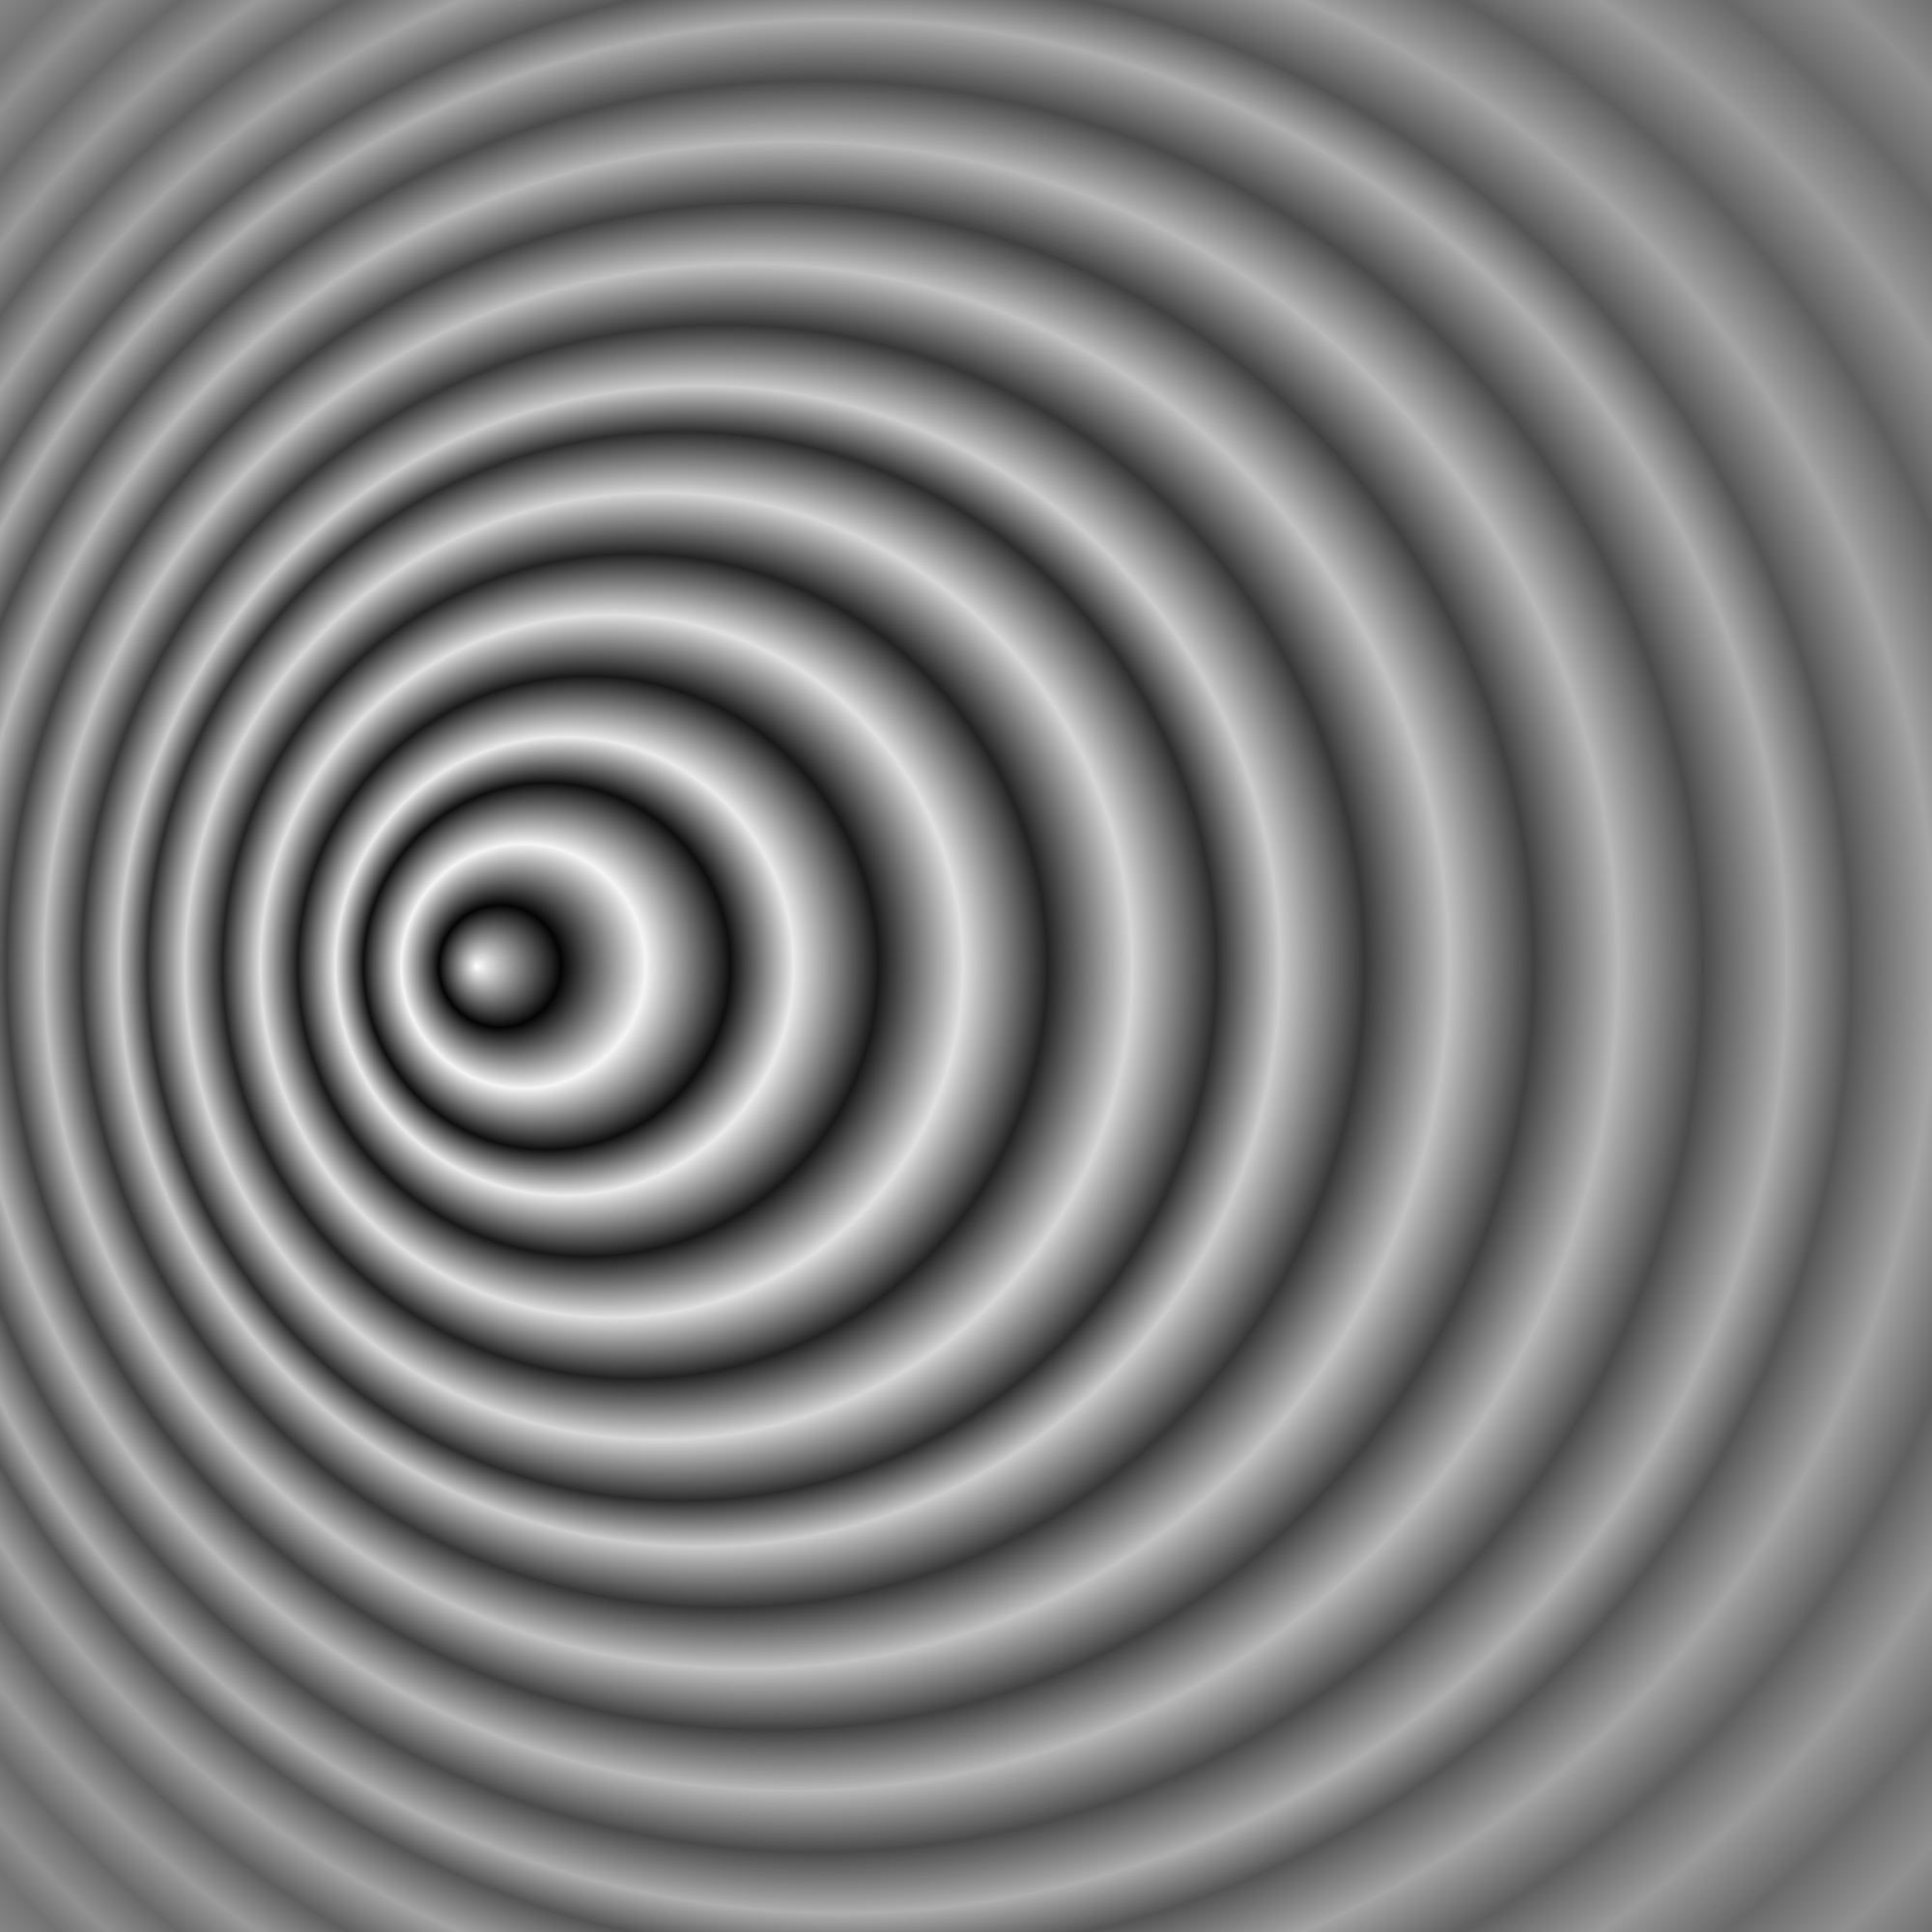
\includegraphics[width=.76\textwidth]{doppler}
        \end{center}
    \end{columns}
\end{frame}

\begin{frame}
    \frametitle{Eliminando o Auto-Bloqueio}

    Solução do artigo:
    \begin{itemize}
        \item Hardware e software \alert{co-design}
        \item Nova tag RFID: \alert{reflete harmônicos} do sinal recebido
        \item Algoritmo HMFCW: seleciona \alert{grupos de frequências}
    \end{itemize}

    \pause

    \begin{center}
        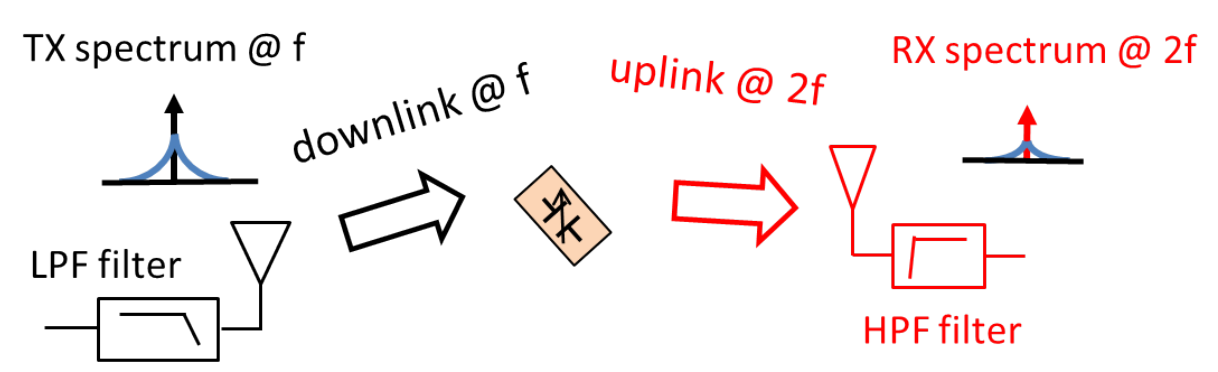
\includegraphics[width=.8\textwidth]{nonlinear-secondharmonic}
    \end{center}
\end{frame}

\subsection{Determinando a Variação de Frequências}
\begin{frame}
    \frametitle{Determinando a Variação de Frequências: Intuição}
    Problema:
    \begin{itemize}
        \item Como determinar corretamente a \alert{fase da reflexão}?
    \end{itemize}
    \begin{align*}
        d_{i}&,d_{j}: \; \text{distância da tag às antenas $i$ e $j$} \\
        \theta& \in [0, 2\pi)\\
        d_{ij} & = d_i - d_j \\
        d_{ij} & = \dfrac{\theta}{2\pi} \dfrac{\lambda}{2} + \alert{n} \dfrac{\lambda}{2}
    \end{align*}

    \pause

    \begin{center}
        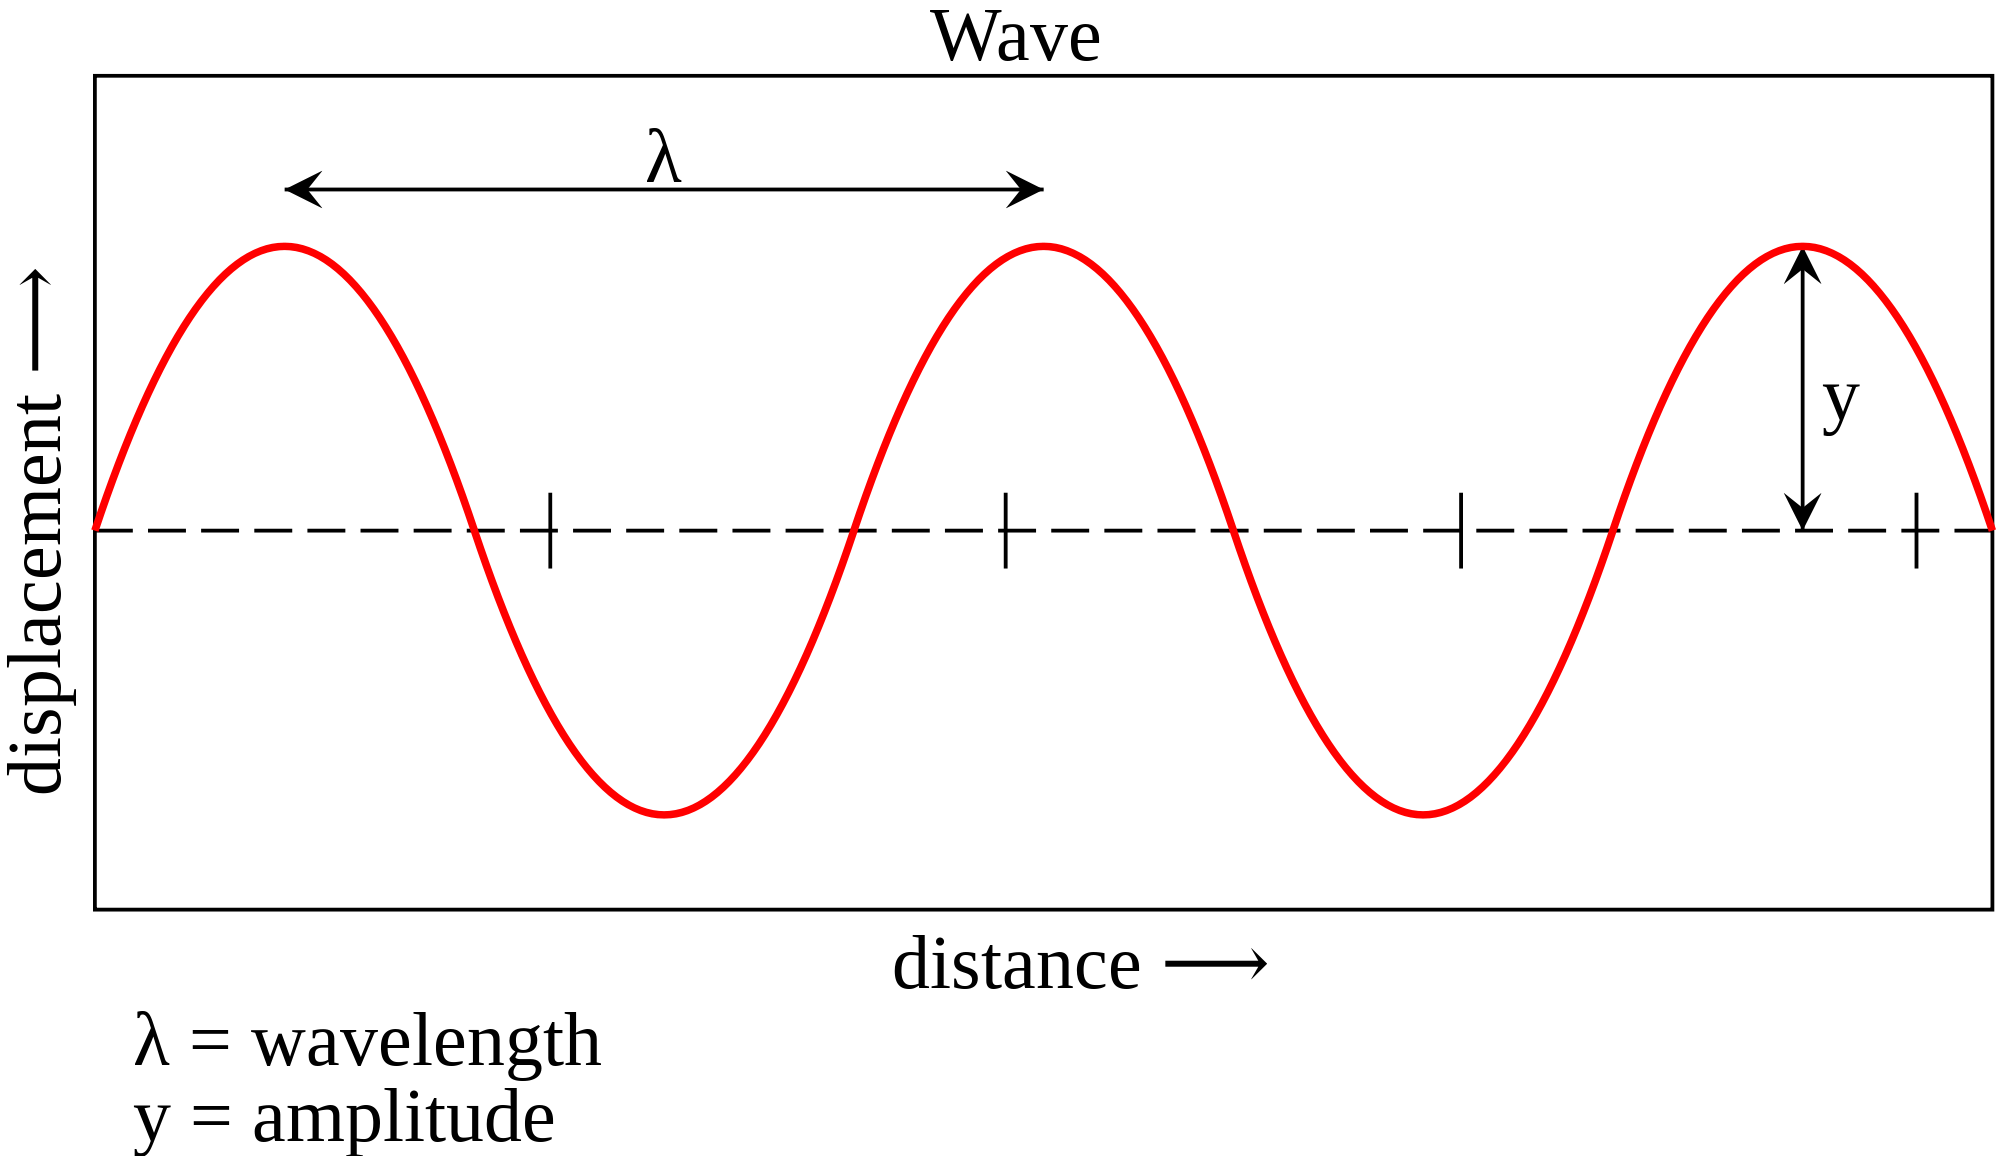
\includegraphics[width=.45\textwidth]{wave}
    \end{center}
\end{frame}

\begin{frame}
    \frametitle{Determinando a Variação de Frequências}

    Solução do artigo:
    \begin{itemize}
        \item \alert{Heuristic optimized continuous wave ranging} (HMFCW)
        \item \alert{Emitir simultaneamente um conjunto de frequências}
    \end{itemize}

    \pause

    \metroset{block=fill}
    \begin{block}{Provam que:}
        Usando uma \alert{combinação de frequências} é possível calcular $\alert{n}$ corretamente,
        desde que os \alert{erros de medição} e a \alert{distância} sejam \alert{limitados},
        e que a \alert{largura de banda seja grande o suficiente}.
    \end{block}
\end{frame}

\begin{frame}
    \frametitle{Determinando a Variação de Frequências}
    Como determinar a combinação de frequências?
    \begin{center}
        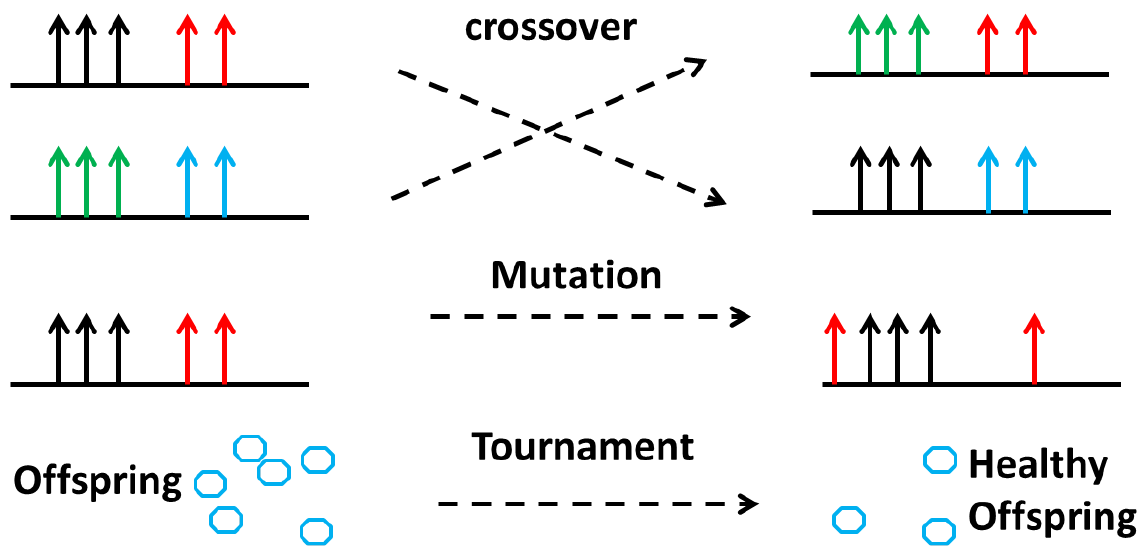
\includegraphics[width=.8\textwidth]{gas}
    \end{center}
\end{frame}

\subsection{Algoritmo de Localização 3D}
\begin{frame}
    \frametitle{Algoritmo de Localização 3D}
    Usando apenas \alert{duas antenas}:

    \begin{center}
        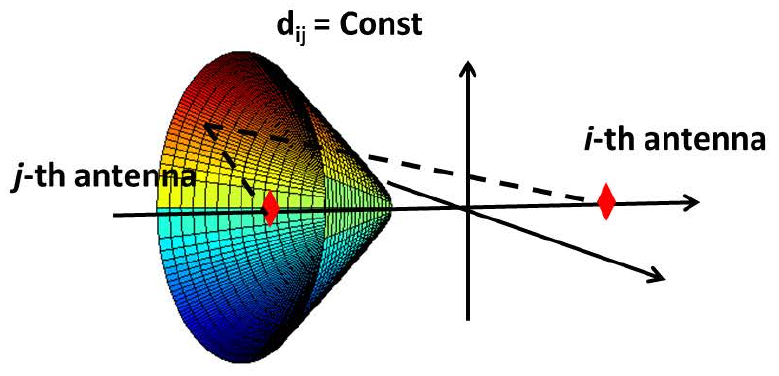
\includegraphics[width=.8\textwidth]{single-hyperboloid}
    \end{center}
\end{frame}

\begin{frame}
    \frametitle{Algoritmo de Localização 3D}
    \begin{center}
        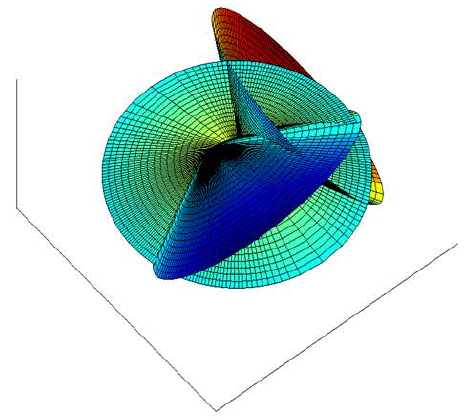
\includegraphics[width=.45\textwidth]{multiple-hyperboloids}
    \end{center}

    Como encontrar a \alert{intersecção dos hiperboloides}?
    \begin{itemize}
        \item Método \alert{Nonlinear Conjugate Gradient}
        \item Fórmula de \alert{Fletcher-Reeves}
        \item \alert{Geração aleatória do ponto inicial}
    \end{itemize}
\end{frame}
